\section{Logical approaches to movement}%
\label{sec:movement-and-quantifier-raising}
\todo{Discuss: division of labour---do you want to analyse a phenomeon
as syntactic or as semantic?}
\todo{Discuss: the $q(A,B,C)$ operator as specification of
  quantification as a syntactic phenomenon.}
\todo{Discuss: tweaking the polarities to obtain scope ambiguity.}

In this section, we will discuss logical approaches to
quantification. We will start out by describing the problem of
quantification. Then we will discuss the choice between semantic and
syntactic approaches. Next, we will discuss the existing semantic
approaches to quantifier raising, and why they are inadequate. We will
then discuss various syntactic approaches to quantifier raising, and
finish by making our own contributions.

\subsection{Quantification in natural language}
Quantification is the problem of analysing scope-taking expressions in
natural language. For instance, the canonical interpretation for a
sentence such as ``Everyone laughs'' is:
\[
  \forall{x}.\PERSON(x)\supset\LAUGH(x)
\]
The problem here, is that the quantifier ``everyone'' is ostensibly an
NP. However, in the given semantics, it is taking scope over
``laughs''. A more obvious version of this problem can be seen in
``John [saw everyone]'', where the quantifier is more deeply nested in
the parse tree:
\[
  \forall{y}.\PERSON(y)\supset\PAST(\SEE(\JOHN,y))
\]
The problem becomes even more interesting when you consider sentences
with multiple quantifiers. Here we observe a phenomenon known as
\emph{scope ambiguity}. The canonical example is the phrase ``Everyone
loves someone'', which has the following interpretations:
\begin{alignat*}{3}
  &\forall x.\PERSON(x) \,&\supset \,&\exists y.\PERSON(y) \,&\wedge  \,&\LIKE(x,y)\\
  &\exists y.\PERSON(y) \,&\wedge  \,&\forall x.\PERSON(x) \,&\supset \,&\LIKE(x,y)
\end{alignat*}

There are several easy ways to obtain these semantics within the
type-logical grammar that we have established in
\autoref{sec:introduction} and \autoref{sec:lexical-ambiguity}.
One approach, due to \citet{montague1973}, is to assign NP the
semantic type $(\e\t)\t$. This way, we can define the lexicon as
follows:
\begin{alignat*}{3}
  &\text{john}     &&= \lambda k. k\;\JOHN                          \\
  &\text{everyone} &&= \lambda k. \forall x. \PERSON(x)\supset k\;x \\
  &\text{laughs}   &&= \lambda x. x\;\LAUGH
\end{alignat*}
We can even build in scope ambiguity by assigning ``loves'' an
  ambiguous type---e.g., using the extension from
  \autoref{sec:lexical-ambiguity}, we assign it the type $\TV\&\TV$,
  and define it as:
\[
  \text{loves} = \lambda k_2. \lambda k_1.
  (k_1\;(\lambda x.k_2\;(\lambda y.\LOVE(x,y))), k_2\;(\lambda y.k_1\;(\lambda x.\LOVE(x,y)))
\]
However, somehow it feels wrong to manually build scope ambiguity into
every verb: it is a universal property of language, so it should not
be encoded in the lexicon, but in our type-logical grammar.

It is also quite odd that we give ``john''---which by all measures is
not a quantifier---the freedom to act as a quantifier. And because we
do not distinguish between quantificational and non-quantificational
NPs, we are left with a large amount of scope ambiguity---spurious
ambiguity. For instance, the sentences ``Mary likes John'' will be
considered ambiguous, with both interpretations equal to $\LIKE(\MARY,
\JOHN)$. \citet{hendriks1993} a solution to this problem, developing a
framework in which terms are lifted into quantificational terms only
when this is needed.
\todo{How does \citet{hendriks1993} deal with scope ambiguity?}

\vspace*{1\baselineskip}

Another approach---popular in associative Lambek calculi---is to use
higher-order syntactic types. For instance, we can assign ``everyone''
the syntactic type $\S\impl\IV$. This also gives us the semantic type
$(\e\t)\t$, and therefore we are able to assign it the same term as
before. This works perfectly for sentences with subject-quantifiers,
and it \emph{does} distinguish between quantificational and
non-quantificational NPs, but it has one downside: it does not work
for sentences with object-quantifiers.
In the \emph{associative} Lambek calculus, we can use the similar
looking type $(\S\impl\NP)\impr\S$---a similarity which extended the
popularity of the associative Lambek calculus way past its due
date. Meanwhile, in NL, we have to devise a type which actually
reflects the sentence structure, such as $\TV\impr\IV$. Using
this type, we can assign ``everyone'' a second interpretation:
\[
  \text{everyone} = \lambda k.\lambda x.\forall y.\PERSON(y)\supset(k\;y\;x)
\]
The need for multiple definitions for `everyone' aside, there are more
problems with this approach: with our current definitions for
``everyone''---and similar definitions for ``someone''---we can only
derive the first of the two expected interpretations for ``Everyone
likes someone''.
Now, we could imagine giving a third definition for ``everyone'' and
``someone'', with the type $(\TV\impr((\S\impl\IV)\impr\IV))$, which
would allow us to define object quantifiers taking scope over subject
quantifiers. However, there are many other cases---think of
ditransitive verbs, or verb phrases modified by some number of
adverbs. Clearly, this is not an elegant solution, as we are basically
hard-coding the structures that quantifiers can take scope over in
their types.

\vspace*{1\baselineskip}

One interesting aspect of the two approaches we have discussed so far
is that they very clearly divide in a semantic and a syntactic
approach. The first approach was implemented in the translation to
semantic types, and in the lexicon. The second approach was
implemented entirely within the syntactic calculus. With any
linguistic phenomenon this is an important question: do we consider it
to be syntactic or semantic in nature? With quantification, the
community seems divided. In this thesis, we will approach the problem
of quantification as a syntactic phenomenon. Therefore, in the
next section we will discuss some of the approaches to quantification
as a semantic problem, and their limitations. Following this, we will
discuss various approaches to quantification as a syntactic problem,
discuss their weaknesses, and try to amend these.

\begin{comment}
In the following section, we will discuss semantic approaches to the
problem of quantification and why these solutions are generally
inadequate.
Next, we will discuss the approach to quantification taken by
\citet{barker2007}. We will then reformulate this approach as an
extension of display NL that maintains the properties we are
interested in---i.e. admissibility of cut, and a decidable and
complete proof search procedure. In \autoref{sec:scope-islands} we
will discuss an extension which can be used to treat a phenomenon
known as `scope islands'. And finally, we will discuss some other
forms of movement---infixation and extraction---and show how they can
be used to analyse sentences with gaps.

\subsubsection{Continuation-Passing Style}
\citet{barker2002,barker2004} advocates the use of continuations in
natural language semantics. He does this with several case studies,
one of which is quantification. The gist of this is as follows:

As mentioned before, the utterance ``John saw everyone,'' the
function-argument structure `(sees everyone) john', but we associate
it with the interpretation $\forall
x.\PERSON(x)\supset\SEE(\JOHN,x)$. This means that the expression
`everyone,' which is deeply nested in the parse tree, must somehow
scope over the entire expression.
\citeauthor{barker2004} proposes to solve this problem by applying a
non-recursive continuation-passing style (CPS) translation to the
lexicon. He lifts expressions of type $A$ into the type $(A\ra R)\ra
R$ for some answer type $R$:
\begin{alignat*}{3}
  &\text{john}     &&= \lambda k. k\;\JOHN\\
  &\text{sees}     &&= \lambda k. k\;\SEE
  \intertext{%
    He then uses this freedom to define `everyone' as a lifted expression
    of type `\e', with $R$ instantiated to `\t':
  }
  &\text{everyone} &&= \lambda k. \forall x.\PERSON(x)\supset k\;x
\end{alignat*}
In addition, he defines a translation on terms, replacing function
application with a method of combining CPS-translated terms:\footnote{%
  It should be noted that \citeauthor{barker2004}'s initial solution
  uses some directional information to ensure that scope-takers are
  always processed in a left-to-right order, instead of always
  processing the argument first, as it is presented here.
  This distinction, however, becomes irrelevant once he introduces the
  ambiguous translation, and therefore I have chosen not to include it.
}
\[
  \overline{M\;N}= \lambda k. \overline{N}\;(\lambda
  n.\overline{M}\;(\lambda m.k\;(m\;n)))
\]

However, the analysis of quantification as a semantic phenomenon has
several issues. The first of these is already mentioned by
\citet{barker2004}: scope ambiguity. The sentence ``Everyone likes
someone'', is ambiguous:
\begin{alignat*}{3}
  &\forall x.\PERSON(x) \,&\supset \,&\exists y.\PERSON(y) \,&\wedge  \,&\LIKE(x,y)\\
  &\exists y.\PERSON(y) \,&\wedge  \,&\forall x.\PERSON(x) \,&\supset \,&\LIKE(x,y)
\end{alignat*}
The solution provided by \citet{barker2002,barker2004} will only
derive the first of these meanings. Barker solves this problem by
adding another possible translation for function application, thereby
making the CPS-translation ambiguous:
\begin{alignat*}{3}
  &\overline{M\;N} &&= \lambda k. \overline{N}\;(\lambda
  n.\overline{M}\;(\lambda m.k\;(m\;n)))\\
  &\overline{M\;N} &&= \lambda k. \overline{M}\;(\lambda
  m.\overline{N}\;(\lambda n.k\;(m\;n)))
\end{alignat*}
There are several problems with this solution. First of all, this
results in a huge amount of spurious ambiguity. A sentence with $n$
words has $n-1$ function applications, and will therefore have
$2^{(n-1)}$ ``different'' interpretations. However, the ambiguity is
only relevant for scope-takers. In the motivating example, ``likes''
is not a scope taker. Nevertheless, there are two possible
translations for ``likes someone'', resulting in \emph{four}
interpretations for the sentence where we only want two.

Secondly, using an ambiguous translation clearly makes our
CPS-translation incompatible with our monadic translation, unless we
are willing to ambiguously translate all our effects. But doing so is
risky, as a right-to-left interpretation may not be desirable for
effects other than quantification. For instance, a right-to-left
interpretation of the state monad for anaphora resolution will allow
sentences such as ``He$_i$ gave a book to John$_i$.''

\vspace*{1\baselineskip}

In more recent work, \citet{moortgat2009,moortgat2012} integrate CPS-semantics into
the syntactic calculus. The result is the Lambek-Grishin (LG)
calculus, a bilinear variant of NL, with semantics inspired on
\citeauthor{parigot1992}'s $\lambda\mu$-calculus
(\citeyear{parigot1992}). LG is a beautifully symmetric calculus, and
display NL, as used in this thesis is, is directly based from it. The
integrated CPS-semantics give some interesting opportunities, for
instance the ability to give quantifiers such as `everyone' the type
$(NP\oslash N)\otimes N$---a pair of a determiner and a noun---and
give them the desired scope-taking semantics.

\vspace*{1\baselineskip}

\citepos{barker2004} CPS-translation and \citepos{moortgat2012}
CPS-semantics both suffer from two related problems:
\begin{enumerate}
\item Both require a \emph{static} choice of answer type. This
  means that the answer type cannot change throughout the
  program. However, there are examples which demonstrate the need for
  allowing dynamic answer types.
\item Both cannot encode \emph{delimiters} past which a nested
  expression cannot take scope. However, in natural language we find
  evidence for scope islands\footnote{%
    We will discuss scope islands in
    \autoref{sec:movement-and-quantifier-raising}.
  }, from which quantifiers cannot escape.
\end{enumerate}
These are the hallmark of \emph{delimited} or \emph{composable}
continuations \citep{danvy1990}. However, while delimited
continuations seem extremely promising, they are still not entirely
without problems. They still suffer from the problem of ambiguity, as
described above for CPS- and monadic translations. Additionally, they
do not form a monad. Instead, they form something known as an indexed
monad, which has two additional type-level parameters, meaning $\eta$
and $\star$ get the following types:
\todo{Remove references to monads.}
\[
  \eta : A\ra\mathbb{M}\;i\;i\;A
  \qquad
  \star: (A\ra\mathbb{M}\;j\;k\;B)\ra\mathbb{M}\;i\;j\;A\ra\mathbb{M}\;i\;k\;B
\]
This makes sense: since we now allow the answer type of the
continuation to change, we need to add indices to keep track of the
input and output answer type. However, the downside of this is that
since we need these additional parameters, we cannot simply
CPS-translate to delimited continuations---if we use a delimited
continuation indexed monad in our semantics, this will have to be
reflected in our syntactic calculus.

While such a solution using delimited continuations may still be
interesting to examine, we will choose to keep our solution entirely
syntactic. In the next section we will present quantifier movement and
scope islands in the syntactic calculus, based on work by
\citet{moortgat1996}, \citet{barker2007} and \citet{barker2015}.

\subsubsection{NL$_\lambda$, NL$_{\text{CL}}$ and NL$_{\text{IBC}}$}
\label{sec:nl-lambda-nl-cl-and-nl-ibc}

\citet{barker2007} and \citet{barker2015} describe an extension to NL
which they call NL$_\lambda$ or NL$_{\text{QR}}$. The main
contribution of this extension is the idea to encode quantifier
raising








In their \citeyear{barker2015} book, \citeauthor{barker2015} describe
an extension of NL which they call NL$_\lambda$. The main insight in
the formulation of this calculus was this: in type-logical grammar,
the antecedent encodes a constituency tree, therefore we can simply
encode quantifier raising in our logic.
\begin{center}
  \vspace*{0.5\baselineskip}
  \begin{minipage}{0.3\linewidth}
    \begin{tikzpicture}
      \Tree [ john [ likes everyone ] ]
    \end{tikzpicture}
  \end{minipage}%
  \begin{minipage}{0.02\linewidth}
    $\equiv$
  \end{minipage}%
  \begin{minipage}{0.4\linewidth}
    \begin{tikzpicture}
      \Tree [ everyone [ $\lambda x.$ [ john [ likes x ] ] ] ]
    \end{tikzpicture}
  \end{minipage}
\end{center}
To achieve this, they add a new modality to NL---that is to say, a
copy of the rules for $\{\impr,\prod,\impl\}$ applying to three new
connectives $\{\himpr,\hprod,\himpl\}$---and the following (somewhat
controversial) equivalence on structures:
\[
  \Sigma[\Delta]\equiv\Delta\circ\lambda x.\Sigma[x]
\]
This equivalence is intuitive, and works as expected. For instance,
using display NL extended with this equivalence, we can easily give a
derivation for ``John likes everyone,'' using the type
$\S\himpl(\NP\himpr\S)$ for quantifiers:
\begin{pfblock}
  \AXC{$\vdots$}\noLine
  \UIC{$\struct{\NP}\prod\struct{(\NP\impr\S)\impl\NP}\prod\struct{\NP}
    \fCenter\struct{\S}$}
  \RightLabel{$\lambda$}
  \UIC{$\struct{\NP}\hprod\lambda{x}.
    (\struct{\NP}\prod\struct{(\NP\impr\S)\impl\NP}\prod x)\fCenter\struct{\S}$}
  \RightLabel{Res$\hprod\himpr$}
  \UIC{$\lambda{x}.(\struct{\NP}\prod\struct{(\NP\impr\S)\impl\NP}\prod{x})
    \fCenter\struct{\NP}\himpr\struct{\S}$}
  \RightLabel{R$\himpr$}
  \UIC{$\lambda{x}.(\struct{\NP}\prod\struct{(\NP\impr\S)\impl\NP}\prod{x})
    \fCenter\struct{\NP\himpr\S}$}
  \AXC{}\RightLabel{Ax}\UIC{$\struct{S}\fCenter\struct{S}$}
  \BIC{$\struct{\S\himpl(\NP\himpr\S)}\fCenter\struct{\S}\himpl\lambda{x}.
    (\struct{\NP}\prod\struct{(\NP\impr\S)\impl\NP}\prod x)$}
  \RightLabel{Res$\himpl\:\hprod$}
  \UIC{$\struct{\S\himpl(\NP\himpr\S)}\hprod\lambda{x}.
    (\struct{\NP}\prod\struct{(\NP\impr\S)\impl\NP}\prod x)\fCenter\struct{\S}$}
  \RightLabel{$\lambda$}
  \UIC{$\struct{\NP}\prod\struct{(\NP\impr\S)\impl\NP}\prod\struct{\S\himpl
      (\NP\himpr\S)}\fCenter\struct{\S}$}
\end{pfblock}
Note that contrary to most linguistic frameworks, in which quantifier
movement is strictly upwards (i.e.\ quantifier raising), in this
framework it ends up being characterised by upwards movement followed
by downwards movement \emph{along the same path}---i.e.\ scope-taking
followed by the insertion of the newly bound variable.

One problem with this framework, however, is the use of a binding
construct in the syntax for structures, which makes it quite difficult
to formalise.
In addition, if we take the equivalence at face value, we end up with
a logic in which we can do all kinds of unpleasant things. For
instance, since contexts are defined as structures with a hole, we
could raise quantifiers past one another, indefinitely:
\begin{pfblock}
  \AXC{$\vdots$}\noLine
  \UIC{$\struct{{\S\impl(\NP\impr\S)}}\hprod\lambda{z}.(\struct{{\S\impl(\NP\impr\S)}}\hprod\lambda{y}.({z}\hprod\lambda{x}.({y}\prod\struct{(\NP\impr\S)\impl\NP}\prod{x})))\fCenter\struct{\S}$}
  \RightLabel{$\lambda$}
  \UIC{$\struct{{\S\impl(\NP\impr\S)}}\hprod\lambda{y}.(\struct{{\S\impl(\NP\impr\S)}}\hprod\lambda{x}.({y}\prod\struct{(\NP\impr\S)\impl\NP}\prod{x}))\fCenter\struct{\S}$}
  \RightLabel{$\lambda$}
  \UIC{$\struct{{\S\impl(\NP\impr\S)}}\hprod\lambda{x}.(\struct{{\S\impl(\NP\impr\S)}}\prod\struct{(\NP\impr\S)\impl\NP}\prod{x})\fCenter\struct{\S}$}
  \RightLabel{$\lambda$}
  \UIC{$\struct{{\S\impl(\NP\impr\S)}}\prod\struct{(\NP\impr\S)\impl\NP}\prod\struct{{\S\impl(\NP\impr\S)}}\fCenter\struct{\S}$}
\end{pfblock}
Or, as \citet{barker2015} note, we could lift variables out of the
scope of their binder:
\begin{pfblock}
  \AXC{$\vdots$}\noLine
  \UIC{${x}\hprod\lambda{y}.(\struct{{\S\impl(\NP\impr\S)}}\hprod\lambda{x}.(\struct{{\S\impl(\NP\impr\S)}}\prod\struct{(\NP\impr\S)\impl\NP}\prod{y}))\fCenter\struct{\S}$}
  \RightLabel{$\lambda$}
  \UIC{$\struct{{\S\impl(\NP\impr\S)}}\hprod\lambda{x}.(\struct{{\S\impl(\NP\impr\S)}}\prod\struct{(\NP\impr\S)\impl\NP}\prod{x})\fCenter\struct{\S}$}
  \RightLabel{$\lambda$}
  \UIC{$\struct{{\S\impl(\NP\impr\S)}}\prod\struct{(\NP\impr\S)\impl\NP}\prod\struct{{\S\impl(\NP\impr\S)}}\fCenter\struct{\S}$}
\end{pfblock}
Needless to say, any logic extended with this equivalence loses a
number of pleasant properties, one of which is decidable proof
search. However, in chapter 17 of their book, \citeauthor{barker2015}
do a great job of capturing the essence of the $\lambda$-rule in a
logical manner---though their system is undecidable. They extend NL by
a second modality $\{\himpr,\hprod,\himpl\}$, add three primitive
structural constants $\{\I,\B,\C\}$, and add the following structural
rules:
\[
  \begin{aligned}
    &\I &&\equiv\lambda x.x           \\
    &\B &&\equiv\lambda x y z.x (y z) \\
    &\C &&\equiv\lambda x y z.x  z y
  \end{aligned}
\]
\begin{center}
  \begin{pfbox}
    \AXC{$X\fCenter Y$}
    \doubleLine\RightLabel{\I}
    \UIC{$X\hprod\I\fCenter Y$}
  \end{pfbox}
  \begin{pfbox}
    \AXC{$X\prod(Y\hprod Z)\fCenter W$}
    \doubleLine\RightLabel{\B}
    \UIC{$Y\hprod((\B\prod X)\prod Z)\fCenter W$}
  \end{pfbox}
  \begin{pfbox}
    \AXC{$(X\hprod Y)\prod Z\fCenter W$}
    \doubleLine\RightLabel{\C}
    \UIC{$X\hprod((\C\prod Y)\prod Z)\fCenter W$}
  \end{pfbox}
\end{center}
\begin{center}
  \begin{pfbox}
    \AXC{$X\fCenter Y$}
    \doubleLine\RightLabel{\I}
    \UIC{$\I\hprod X\fCenter Y$}
  \end{pfbox}
  \begin{pfbox}
    \AXC{$X\prod(Z\hprod Y)\fCenter W$}
    \doubleLine\RightLabel{\B}
    \UIC{$((\B\prod X)\prod Z)\hprod Y\fCenter W$}
  \end{pfbox}
  \begin{pfbox}
    \AXC{$(Y\hprod X)\prod Z\fCenter W$}
    \doubleLine\RightLabel{\C}
    \UIC{$((\C\prod Y)\prod Z)\hprod X\fCenter W$}
  \end{pfbox}
\end{center}
\begin{center}
  \begin{pfbox}
    \AXC{$X\fCenter Y$}
    \doubleLine\RightLabel{\I}
    \UIC{$\I\hprod X\fCenter Y$}
  \end{pfbox}
  \begin{pfbox}
    \AXC{$X\prod(Y\hprod Z)\fCenter W$}
    \doubleLine\RightLabel{\B}
    \UIC{$((\B\prod X)\prod Y)\hprod Z\fCenter W$}
  \end{pfbox}
  \begin{pfbox}
    \AXC{$(X\hprod Z)\prod Y\fCenter W$}
    \doubleLine\RightLabel{\C}
    \UIC{$((\C\prod X)\prod Y)\hprod Z\fCenter W$}
  \end{pfbox}
\end{center}
They call the result NL$_{\text{CL}}$ (and, occasionally,
NL$_{\text{IBC}}$). In this calculus, quantifier raising can be done
in much the same way as in NL$_\lambda$---though the new version is
ever so slightly more verbose:\footnote{%
  Inverted applications of the \I, \B\ and \C\ rules are marked with a prime.
}
\begin{pfblock}
  \AXC{$\vdots$}\noLine
  \UIC{$\struct{\NP}\prod\struct{(\NP\impr\S)\impl\NP}\prod\struct{{\NP}}\fCenter\struct{{\S}}$}
  \RightLabel{Res$\prod\impr$}
  \UIC{$\struct{(\NP\impr\S)\impl\NP}\prod\struct{{\NP}}\fCenter\struct{\NP}\impr\struct{{\S}}$}
  \RightLabel{Res$\prod\impr$}
  \UIC{$\struct{{\NP}}\fCenter\struct{(\NP\impr\S)\impl\NP}\impr\struct{\NP}\impr\struct{{\S}}$}
  \RightLabel{\I}
  \UIC{$\struct{{\NP}}\hprod\I\fCenter\struct{(\NP\impr\S)\impl\NP}\impr\struct{\NP}\impr\struct{{\S}}$}
  \RightLabel{Res$\impr\prod$}
  \UIC{$\struct{(\NP\impr\S)\impl\NP}\prod(\struct{{\NP}}\hprod\I)\fCenter\struct{\NP}\impr\struct{{\S}}$}
  \RightLabel{\B}
  \UIC{$\struct{{\NP}}\prod((\B\prod\struct{(\NP\impr\S)\impl\NP})\prod\I)\fCenter\struct{\NP}\impr\struct{{\S}}$}
  \RightLabel{Res$\prod\impr$}
  \UIC{$\struct{\NP}\prod(\struct{{\NP}}\hprod((\B\prod\struct{(\NP\impr\S)\impl\NP})\prod\I))\fCenter\struct{{\S}}$}
  \RightLabel{\B}
  \UIC{$\struct{{\NP}}\hprod((\B\prod\struct{\NP})\prod((\B\prod\struct{(\NP\impr\S)\impl\NP})\prod\I))\fCenter\struct{{\S}}$}
  \RightLabel{Res$\hprod\himpr$}
  \UIC{$((\B\prod\struct{\NP})\prod((\B\prod\struct{(\NP\impr\S)\impl\NP})\prod\I))\fCenter\struct{{\NP}}\himpr\struct{{\S}}$}
  \RightLabel{R$\himpr$}
  \UIC{$((\B\prod\struct{\NP})\prod((\B\prod\struct{(\NP\impr\S)\impl\NP})\prod\I))\fCenter\struct{{\NP\himpr\S}}$}
  \AXC{}\RightLabel{Ax}\UIC{$\struct{\S}\fCenter\struct{{\S}}$}
  \RightLabel{L$\himpl$}
  \BIC{$\struct{{\S\himpl(\NP\himpr\S)}}\fCenter\struct{\S}\himpl((\B\prod\struct{\NP})\prod((\B\prod\struct{(\NP\impr\S)\impl\NP})\prod\I))$}
  \RightLabel{Res$\himpl\:\hprod$}
  \UIC{$\struct{{\S\himpl(\NP\himpr\S)}}\hprod((\B\prod\struct{\NP})\prod((\B\prod\struct{(\NP\impr\S)\impl\NP})\prod\I))\fCenter\struct{\S}$}
  \RightLabel{$\B'$}
  \UIC{$\struct{\NP}\prod(\struct{{\S\himpl(\NP\himpr\S)}}\hprod((\B\prod\struct{(\NP\impr\S)\impl\NP})\prod\I))\fCenter\struct{\S}$}
  \RightLabel{Res$\prod\impr$}
  \UIC{$\struct{{\S\himpl(\NP\himpr\S)}}\hprod((\B\prod\struct{(\NP\impr\S)\impl\NP})\prod\I)\fCenter\struct{\NP}\impr\struct{\S}$}
  \RightLabel{$\B'$}
  \UIC{$\struct{(\NP\impr\S)\impl\NP}\prod(\struct{{\S\himpl(\NP\himpr\S)}}\hprod\I)\fCenter\struct{\NP}\impr\struct{\S}$}
  \RightLabel{Res$\impr\prod$}
  \UIC{$\struct{{\S\himpl(\NP\himpr\S)}}\hprod\I\fCenter\struct{(\NP\impr\S)\impl\NP}\impr\struct{\NP}\impr\struct{\S}$}
  \RightLabel{$\I'$}
  \UIC{$\struct{{\S\himpl(\NP\himpr\S)}}\fCenter\struct{(\NP\impr\S)\impl\NP}\impr\struct{\NP}\impr\struct{\S}$}
  \RightLabel{Res$\prod\impr$}
  \UIC{$\struct{(\NP\impr\S)\impl\NP}\prod\struct{{\S\himpl(\NP\himpr\S)}}\fCenter\struct{\NP}\impr\struct{\S}$}
  \RightLabel{Res$\prod\impr$}
  \UIC{$\struct{\NP}\prod\struct{(\NP\impr\S)\impl\NP}\prod\struct{{\S\himpl(\NP\himpr\S)}}\fCenter\struct{\S}$}
\end{pfblock}

One of the advantages of this formalisation is that it gets rid of the
awkward binding construct in the syntax of structures. In addition, it
makes it clear that quantifiers can only move past \emph{solid}
products. However, it is not entirely free of problems. One of the
more glaring problems is that using this encoding, any expression can
be the subject of quantifier raising. For instance, in ``John likes
Mary,'' we could choose to raise the verb:
\begin{pfblock}
  \AXC{$\vdots$}\noLine
  \UIC{$\struct{{(\NP\impr\S)\impl\NP}}\hprod(\B\prod\struct{\NP})
    \prod((\C\prod\I)\prod\struct{\NP})\fCenter\struct{\S}$}\noLine
  \UIC{$\vdots$}\noLine
  \UIC{$\struct{\NP}\prod\struct{{(\NP\impr\S)\impl\NP}}\prod\struct{\NP}\fCenter\struct{\S}$}
\end{pfblock}
Since verbs are usually not considered scope-takers, it is unlikely
that raising the verb would lead to anything other then lowering it
again. However, the fact that we leave it open as an opportunity is
wasted computational effort; while all futile attempts at raising and
lowering will lead to a loop, and therefore spare us the spurious
ambiguity, there are still a great deal of futile attempts to be made.

Another problem is the $\I'$-rule. It allows us to introduce an
arbitrary amount of \I's, which causes a \emph{growing} loop in our
proof search procedure:
\begin{pfblock}
  \AXC{$\vdots$}\noLine
  \UIC{$((\struct{\NP}\prod\struct{\NP\impr\S})\hprod\I)\hprod\I\fCenter\struct{\S}$}
  \RightLabel{$\I'$}
  \UIC{$(\struct{\NP}\prod\struct{\NP\impr\S})\hprod\I\fCenter\struct{\S}$}
  \RightLabel{$\I'$}
  \UIC{$\struct{\NP}\prod\struct{\NP\impr\S}\fCenter\struct{\S}$}
\end{pfblock}
I propose to handle both of these issues with one simple addition. The
idea is to add a new unary connective, $\q[A]$, which represents a
license to perform quantifier raising. Since we want to replace the
problematic $\I'$-rule, we will choose the structural version of our
quantifying license to be a \emph{hollow} product with a right-hand
unit. On the other side, since we do not want logical products, we
will keep $\q[A]$ it as an atomic logical connective. This gives us
the following logical left rule:
\begin{pfblock}
  \AXC{$\struct{A}\hprod\I\fCenter Δ$}
  \RightLabel{L\I}
  \UIC{$\struct{\q[A]}\fCenter Δ$}
\end{pfblock}
The appropriate right rule is easily derived from the conventional
display calculus rules for products and units---though I do not imagine
we will generally want to see quantifying licenses in our output type:
\begin{pfblock}
  \AXC{$Γ\fCenter\struct{B}$}
  \RightLabel{R\I}
  \UIC{$Γ\hprod\I\fCenter\struct{\q[B]}$}
\end{pfblock}
And indeed, the pair obeys all constraints imposed by display
calculus, including a valid proof for \textbf{C8}:
\begin{pfblock}
  \AXC{$Γ\fCenter\struct{A}$}
  \AXC{$\struct{A}\hprod\I\fCenter Δ$}
  \RightLabel{Res$\hprod\himpl$}
  \UIC{$\struct{A}\fCenter Δ\himpl\I$}
  \RightLabel{Cut}
  \BIC{$Γ\fCenter Δ\himpl\I$}
  \RightLabel{Res$\himpl\hprod$}
  \UIC{$Γ\hprod\I\fCenter Δ$}
\end{pfblock}
Note that we keep the $\I$-rule, though we rename it $\I^-$ to
emphasise that it can now only \emph{remove} $\I$s. The full
extension, including semantics, and focused rules, can be found in
\autoref{fig:extension-quantifier-raising}. The semantics are rather
trivial: we simply translate all constants as units, and translate
$\q[A]$ as $A$, inserting and removing the right unit as needed.

\begin{figure}[hb]
  \begin{mdframed}
    \centering
    \begin{minipage}{0.666\linewidth}
      \centering
      \begin{alignat*}{4}
        \text{Type}     &  \;&A,B&\coloneqq\ldots\vsep A\himpr B\vsep B\himpl A\vsep\q[A]\\
        \text{Structure}&^+\;&Γ  &\coloneqq\ldots\vsep Γ_1\hprod Γ_2\vsep\I\vsep\B\vsep\C\\
        \text{Structure}&^-\;&Δ  &\coloneqq\ldots\vsep Γ\himpr Δ\vsep Δ\himpl Γ
      \end{alignat*}
    \end{minipage}%
    \begin{minipage}{0.333\linewidth}
      \centering
      \begin{alignat*}{4}
        &\text{Pol}(A\himpr B) &&\mapsto{-}\\
        &\text{Pol}(B\himpl A) &&\mapsto{-}\\
        &\text{Pol}(\q[A])    &&\mapsto{+}
      \end{alignat*}
    \end{minipage}
    \\[1\baselineskip]
    (copy of rules for $\{\impr,\prod,\impl\}$ from
    \autoref{fig:display-calculus} for $\{\himpr,\hprod,\himpl\}$)
    \\[1\baselineskip]
    \begin{pfbox}
      \AXC{$\struct{A}\hprod\I\fCenter Δ$}
      \RightLabel{L\I}
      \UIC{$\struct{\q[A]}\fCenter Δ$}
    \end{pfbox}
    \begin{pfbox}
      \AXC{$Γ\fCenter\focus{B}$}
      \RightLabel{R\I}
      \UIC{$Γ\hprod\I\fCenter\focus{\q[B]}$}
    \end{pfbox}
    \begin{pfbox}
      \AXC{$Γ\fCenter Δ$}
      \RightLabel{$\I^-$}
      \UIC{$Γ\hprod\I\fCenter Δ$}
    \end{pfbox}
    \\[1\baselineskip]
    \begin{pfbox}
      \AXC{$Γ_1\prod(Γ_2\hprod Γ_3)\fCenter Δ$}
      \doubleLine\RightLabel{\B}
      \UIC{$Γ_2\hprod((\B\prod Γ_1)\prod Γ_3)\fCenter Δ$}
    \end{pfbox}
    \begin{pfbox}
      \AXC{$(Γ_1\hprod Γ_2)\prod Γ_3\fCenter Δ$}
      \doubleLine\RightLabel{\C}
      \UIC{$Γ_1\hprod((\C\prod Γ_2)\prod Γ_3)\fCenter Δ$}
    \end{pfbox}
    \\[1\baselineskip]
    \hrulefill
    \\[1\baselineskip]
    {
      \renewcommand{\arraystretch}{1.5}%
      \(\!
      \begin{array}{c c c}
        \multicolumn{3}{c}{\tr[({\q[A]})]\mapsto\tr[A]}\\
        \tr[\I]\mapsto\top      & \tr [\B]\mapsto\top     & \tr [\C]\mapsto\top\\
      \end{array}
      \)
    }
    \\[1\baselineskip]
    (copy of translations for $\{\impr,\prod,\impl\}$ from
    \autoref{fig:display-calculus-to-explicit-lamET} for
    $\{\himpr,\hprod,\himpl\}$)
    \\[1\baselineskip]
    \begin{pfbox}
      \AXC{$x:\struct{A}\hprod\I\fCenter M:Δ$}
      \RightLabel{L\I}
      \UIC{$y:\struct{\q[A]}\fCenter \sub{M}{(y,())}{x}:Δ$}
    \end{pfbox}
    \begin{pfbox}
      \AXC{$x:Γ\fCenter\focus{M:B}$}
      \RightLabel{R\I}
      \UIC{$y:Γ\hprod\I\fCenter\focus{\sub{M}{\fst{y}}{x}:\q[B]}$}
    \end{pfbox}
    \begin{pfbox}
      \AXC{$x:Γ\fCenter M:Δ$}
      \RightLabel{$\I^-$}
      \UIC{$y:Γ\hprod\I\fCenter \sub{M}{\fst{y}}{x}:Δ$}
    \end{pfbox}
    \\[1\baselineskip]
    (where $\fst{x}=\case{x}{y}{z}{y}$)
    \\[1\baselineskip]
    (\B\ and \C\ translate to various combinations of associativity,
    commutativity, $\emptyset$E and weakening)
    \\
    \vspace*{\baselineskip}
  \end{mdframed}
  \caption{
    Extension of calculus in \autoref{fig:display-calculus} which
    supports quantifier raising.}%
  \label{fig:extension-quantifier-raising}
\end{figure}

%%% Local Variables:
%%% mode: latex
%%% TeX-master: t
%%% End:


The extension presented so far for quantifier raising is pretty good:
because we have removed all growing loops in structural rules, it now
has a decidable and complete procedure for proof search, and it neatly
captures quantifier movement---i.e.\ moving upwards, taking scope,
binding a variable, and moving that variable back down. However, it
still has one problem: spurious ambiguity. Imagine a sentence with two
quantifiers $P$ and $Q$, respectively \emph{one} and \emph{two} places
removed from the top of the syntax tree. The ambiguity that we want is
``do we raise $P$ first, or do we raise $Q$ first?'' However, in
addition to these possibilities, we now also have to possibility to
raise $Q$ one step, then raise $P$, and then raise $Q$ a second
step---semantically, this is equivalent to raising $P$, then
$Q$. NL$_\lambda$---if you only allow quantifier raising past solid
products---does not have this problem.

\citet[][chapter 17.6]{barker2015} examine the restrictions that need
to be put on the $\lambda$-rule in order to be able to translate
NL$_\lambda$ to NL$_{\text{CL}}$. In order to keep our structural
rules simple, and our calculus free of structural lambdas, I opt to go
the other way around, and see how close we can get to defining the
$\lambda$-rule in our calculus in \autoref{fig:extension-quantifier-raising}.
For this, we will need the following definitions:
\begin{center}
  $\text{Context}\;Σ\coloneqq\Box\vsep Σ\prodl Γ\vsep Γ\prodr Σ$\\
  \begin{minipage}{0.45\linewidth}
    \begin{alignat*}{2}
      &\Box       \;&&[Γ']\mapsto Γ'\\
      &(Σ\prodl Γ)\;&&[Γ']\mapsto (Σ[Γ']\prod Γ)\\
      &(Γ\prodr Σ)\;&&[Γ']\mapsto (Γ\prod Σ[Γ'])
    \end{alignat*}
  \end{minipage}
  \begin{minipage}{0.45\linewidth}
    \begin{alignat*}{2}
      &\trace(\Box)     \;&&\mapsto \mathbf{I}\\
      &\trace(Σ\prodl Γ)\;&&\mapsto ((\mathbf{C}\prod \trace(Σ))\prod Γ)\\
      &\trace(Γ\prodr Σ)\;&&\mapsto ((\mathbf{B}\prod Γ)\prod
      \trace(Σ))
    \end{alignat*}
  \end{minipage}
\end{center}
First we have contexts, which encode structures with a single hole,
where the nodes leading up to the hole are all solid
products---exactly the type of structure that quantifiers can move up
through. The syntax is a little abusive, as we use the same symbol for
products, products with a hole in their left argument, and products
with a hole in their right argument. However, as we require that
contexts have only a single hole, it is always unambiguous. Note that
products are right-associative.
Secondly, we have the plugging function `$\plug$', which inserts some
structure into the single hole in a context.
Lastly, the `trace' function computes, from a context, the trace of
$\B$s and $\C$s that would be left after something quantifies out of
that context.

Given these definitions, we can show that the following rule for
quantifier movement is admissible, by induction on the structure of
the context:
\begin{pfblock}
  \AXC{$\struct{A}\hprod\trace(Σ)\fCenter Δ$}
  \doubleLine\RightLabel{$\uparrow\downarrow$}
  \UIC{$Σ[\struct{\q[A]}]\fCenter Δ$}
\end{pfblock}
This new rule is very close to \citeauthor{barker2015}'s equivalence,
with as its only difference that the quantifying license is now built
into it:
\[
  \Sigma[\Delta]\equiv\Delta\circ\lambda x.\Sigma[x]
  \qquad
  Σ[\struct{\q[A]}]\equiv\struct{A}\hprod\trace(Σ)
\]
In fact, if you interpret the products as function applications, and
the constants $\{\I,\B,\C\}$ as the combinators, as \citet{barker2015}
intended, then the right-hand side expressions are equivalent.\footnote{%
  As an aside: what we set out to encode were contexts with holes that
  are unique---plugging should never duplicate or forget
  information. So the $\lambda$-terms in NL$_\lambda$ were implicitly
  linear. The combinators $\I$, $\B$ and $\C$ correspond precisely to
  the linear lambda calculus. However, the combinator language is far
  easier to encode than linear binding constructs.
}
Proof search with this derived rule is still complete; it merely
enforces that the entire quantifier raising or lowering is done in one
go.\todo{No proof.}

In their discussion of decidability, \citet{barker2015} derive the
`expansion' and `reduction' rules which more-or-less correspond to
the two directions of the equivalence, or the two directions of our
$\uparrow\downarrow$-rule. They then combine these rules with
L$\himpl$ and R$\himpr$, respectively, yielding the
$\himpl\,\text{L}_\lambda$ and $\himpr\text{R}_\lambda$ rules. The
advantage of these combined rules is that they obey the sub-formula
property, and are therefore suited to naive backward-chaining proof
search. We can do a similar thing using our $\uparrow\downarrow$-rule:
\begin{center}
  \begin{pfbox}
    \AXC{$\trace(Σ)\fCenter\struct{A\himpr B}$} \AXC{$\struct{C}\fCenter Δ$}
    \RightLabel{\qup}
    \BIC{$Σ[\struct{\q[C\himpl(A\himpr B)]}]\fCenter Δ$}
  \end{pfbox}
  \begin{pfbox}
    \AXC{$Σ[\struct{A}]\fCenter\struct{B}$}
    \RightLabel{\qdown}
    \UIC{$\trace(Σ)\fCenter\struct{A\himpr B}$}
  \end{pfbox}
\end{center}
While proof search with these rules is decidable, it is no longer
complete. However, it \emph{is} complete for the fragment of display
NL where all types involving a quantifying license are of the form
$\q[C\himpl(A\himpr B)]$, which is what we can reasonably expect from
natural language.
In addition, proof search using these rules is no longer plagued by
the spurious ambiguity that resulted from the $\B$ and $\C$
rules---and, to boot, we can write proofs involving quantifier
movement in a much more succinct manner:
\begin{pfblock}
  \AXC{$\vdots$}\noLine
  \UIC{$\struct{\NP}\prod\textsc{loves}\prod\struct{\NP}\fCenter\struct{\S}$}
  \RightLabel{\qdown}
  \UIC{$\trace(\Box\prod\textsc{loves}\prod\struct{\NP})\fCenter\struct{{\NP\himpr\S}}$}
  \AXC{}\RightLabel{Ax}\UIC{$\struct{\S}\fCenter\struct{\S}$}
  \RightLabel{\qup}
  \BIC{$\textsc{everyone}\prod\textsc{loves}\prod\struct{\NP}\fCenter\struct{\S}$}
  \RightLabel{\qdown}
  \UIC{$\trace(\textsc{everyone}\prod\textsc{loves}\prod\Box)\fCenter\struct{{\NP\himpr\S}}$}
  \AXC{}\RightLabel{Ax}\UIC{$\struct{\S}\fCenter\struct{\S}$}
  \RightLabel{\qup}
  \BIC{$\textsc{everyone}\prod\textsc{loves}\prod\textsc{someone}\fCenter\struct{\S}$}
\end{pfblock}
\vspace*{-1\baselineskip}
\begin{gather*}
  \downmapsto
  \\
  (\text{someone}\;(\lambda y. \text{everyone}\;(\lambda x.\text{likes}\;y\;x)))
  \\
  \downmapsto
  \\
  \exists y.\PERSON(y)\wedge\forall x.\PERSON(x)\supset\LIKE(x,y)
\end{gather*}
Note that though we have the option, we do not have to unfold the
application of `trace' in this particular proof. In future proofs, if
we choose to fold or unfold an application of `trace', we will
explicitly mark this as an application of rewriting by equality
(`$=$').

\begin{landscape}
  \begin{figure}
    \begin{mdframed}
      \centering
      \begin{pfblock}[0.74]
        \AXC{$\vdots$}\noLine
        \UIC{$
          \textsc{the}\prod\textsc{author}\prod\textsc{of}\prod\struct\NP
          \fCenter\struct\NP$}
        \RightLabel{\qdown}
        \UIC{$
          \trace(\textsc{the}\prod\textsc{author}\prod\textsc{of}\prod\Box)
          \fCenter\struct{\NP\himpl\NP}$}
        \AXC{$\vdots$}\noLine
        \UIC{$
          \NP\prod\textsc{feared}\prod\textsc{the}\prod\textsc{ocean}\fCenter\struct{\S}$}
        \RightLabel{DP}
        \UIC{$
          \textsc{feared}\prod\textsc{the}\prod\textsc{ocean}\fCenter\struct{\NP\impr\S}$}
        \AXC{$\vdots$}\noLine
        \UIC{$\struct{\N\impr\N}\fCenter\textsc{book}\impr\struct\N$}
        \RightLabel{L$\impl$}
        \BIC{$
          \struct{(\N\impr\N)\impl(\NP\impr\S)}
          \fCenter(\textsc{book}\impr\struct\N)\impl
          (\textsc{feared}\prod\textsc{the}\prod\textsc{ocean})$}
        \RightLabel{\qup}
        \BIC{$
          \textsc{the}\prod\textsc{author}\prod\textsc{of}\prod\textsc{which}
          \fCenter(\textsc{book}\impr\struct\N)\impl(\textsc{feared}\prod
          \textsc{the}\prod\textsc{ocean})$}
        \RightLabel{DP}
        \UIC{$
          \textsc{book}\prod(\textsc{the}\prod\textsc{author}\prod\textsc{of}\prod
          \textsc{which})\prod\textsc{feared}\prod\textsc{the}\prod\textsc{ocean}
          \fCenter\struct\N$}
        \AXC{$\vdots$}\noLine
        \UIC{$
          \textsc{alice}\prod\textsc{read}\prod\struct\NP
          \fCenter\struct\S$}
        \RightLabel{\qdown}
        \UIC{$
          \trace(\textsc{alice}\prod\textsc{read}\prod\Box)
          \fCenter\struct{\S\himpl\NP}$}
        \AXC{}\RightLabel{Ax}\UIC{$\struct\S\fCenter\struct\S$}
        \RightLabel{\qup}
        \BIC{$
          \textsc{alice}\prod\textsc{read}\prod\q[(\S\himpl\NP)\himpr\S]
          \fCenter\struct{\S}$}
        \RightLabel{DP}
        \UIC{$
          \q[(\S\himpl\NP)\himpr\S]
          \fCenter\textsc{read}\impr(\textsc{alice}\impr\struct{\S})$}
        \RightLabel{L$\impl$}
        \BIC{$
          \textsc{a}\fCenter(\textsc{read}\impr(\textsc{alice}\impr\struct{\S}))\impl
          (\textsc{book}\prod(\textsc{the}\prod\textsc{author}\prod\textsc{of}\prod
          \textsc{which})\prod\textsc{feared}\prod\textsc{the}\prod\textsc{ocean})$}
        \RightLabel{DP}
        \UIC{$
          \textsc{alice}\prod\textsc{read}\prod\textsc{a}\prod\textsc{book}\prod
          (\textsc{the}\prod\textsc{author}\prod\textsc{of}\prod\textsc{which})\prod
          \textsc{feared}\prod\textsc{the}\prod\textsc{ocean}\fCenter\struct{\S}$}
      \end{pfblock}
      \vspace*{-1\baselineskip}
      \begin{gather*}
        \downmapsto
        \\
        \text{a}\;(\lambda{x}.\text{which}\;
          (\lambda{z}.\text{the}\;(\text{of}\;z\;\text{author}))\;
          (\lambda{w}.\text{fear}\;(\text{the}\;\text{ocean})\;w)\;
          \text{book}\;x)\;
          (\lambda{y}.\text{read}\;y\;\text{alice})
        \\
        \downmapsto
        \\
        \exists{x}.
        (\BOOK(x)\wedge\PAST(\FEAR(\iota(\lambda{y}.\OF(y,\AUTHOR,x)),\iota(\OCEAN)))
        \wedge\PAST(\READ(\ALICE,x))
      \end{gather*}
    \end{mdframed}
    \caption{An example of changing answer types.}
    \label{fig:example-changing-answer-type}
  \end{figure}
\end{landscape}
%
%%% Local Variables:
%%% mode: latex
%%% TeX-master: t
%%% End:


\subsubsection{Parasitic scope}
Parasitic scope is a interesting mechanism, put forward by
\citet{barker2007}, which allows expressions to capture another
quantifier's scope. Using this mechanism, a parasitic expression can
take scope \emph{right} underneath another quantifier, and capture the
bound variable. For instance, a parasitic expression $k$ might take
scope under the bounded quantifier `everyone', receiving both its
context and the bound variable $x$ as arguments:
\[
  \forall{x}.\PERSON(x)\supset(k\ldots{x})
\]
The mechanism depends crucially on two properties:\footnote{%
  Though I do not rule out the possibility that the mechanism can
  exists under different circumstances.
}
\begin{enumerate*}[label=(\arabic*)]
\item quantification must be (at least) a two-step process; and
\item the `function' that becomes the argument of the quantifier must
  be represented in the type.
\end{enumerate*}
NL$_\lambda$ (obviously) respects these requirements: we have
$\himpl\text{L}_\lambda$ (or $\qup$) and $\himpr\text{R}_\lambda$ (or
$\qdown$), and the type of the `function' that is quantifier-over is
represented as ${A}\himpr{B}$. Using this, we can write a quantifier
which targets the type of raised quantifiers. For instance,
\[
  \q[(\NP\himpr\S)\himpl(\ldots\himpr(\NP\himpr\S))]
\]
Canonical examples of such quantifiers are expressions such as `same'
and `different', as used in the sentence ``The same waiter served
everyone'', which \citet{barker2007} assigns more-or-less the
following semantics:\footnote{%
  I suppose that selection of the choice function $f$ should be
  bounded by a predicate such as $\exists{z}.\forall{x}.f(x)=z$, as
  would be dictated by the semantics of same.
}
\[
  \text{everyone}\;(\lambda{X}.\exists{f_{(\e\t)\e}}.\forall{x<X}:
  \PAST(\SERVE(x,\iota(f(\WAITER)))))
\]
\citeauthor{barker2007} describes this as meaning that ``[e]veryone
collectively has the property of being a group such that there is a
unique waiter who served each member of the group''. It is clear that
the intention is to have $x$ range over the same set of variables over
which `everyone' ranges. However, it is not entirely clear to me how
`everyone' should reduce---it is ostensibly not a quantifier, but a
function which takes a continuation and provides it with the set of
all people (e.g.\ $\text{everyone}=\lambda{k}.k\;\PERSON$). All this
seems to be a whole lot of work to push the existential selecting the
choice function up over the quantifier introduced by `everyone'.

\citet{kiselyov2015b} provides much clearer semantics for the semantics
of `same' and `different' sentences:
\[
  \exists{z}.\forall{y}.\PAST(\SERVE(\iota(\lambda{x}.\WAITER(x)\wedge{x=z}),y))
\]
The crucial point seems to be that words such as `same' want to take
scope \emph{over} another quantifier, but in the meantime also want
access to the variable bound by that quantifier. In order to derive
these semantics, we use a different type for parasitic quantifiers---a
double quantifier:
\[
  \q[\S\himpl(\quad{\q[(\NP\himpr\S)\himpl(\quad{\ldots}\quad\himpr(\NP\himpr\S))]}\quad\himpr\S)]
\]
Such double quantification has some interesting aspects. First of all,
one might expect huge amounts of quantifier ambiguity. However,
because a double quantifier has to take scope once \emph{normally} and
once \emph{parasitically}, in the case where there is one double and
one normal quantifier, there is not room for ambiguity. The double
quantifier \emph{has} to take scope first, in order to be able to take
scope parasitically while the other quantifier is taking scope.

In \autoref{fig:parasitic-scope}, we give an analysis of the sentence
``A different waiter served everyone'', for which we derive the
following semantics, also assigned by \citeauthor{kiselyov2015b}:
\begin{align*}
  &\exists{f_{\e\e\t}}.(\forall{x}.\forall{y}.\nexists{z}.f\;z\;x\wedge{f\;z\;y})\;\wedge\\
  &\qquad(\forall{y}.\PERSON(y)\supset(\exists{x}.\WAITER(x)\wedge{f\;y\;x\wedge\PAST(\SERVE(y,x))}))
\end{align*}
The first clause, $\forall{x}.\forall{y}.\nexists{z}.f\;z\;x\wedge
{f\;z\;y}$, is entirely contained withing the semantics for
`different'---it enforces that $f$ does not assign the same output $z$
to two different inputs. The full lexicon used in the derivation is
given in \autoref{fig:parasitic-scope-lexicon}
\begin{figure}[hb]
  \centering
  \begin{mdframed}
    \[
      \renewcommand*{\arraystretch}{1}
      \begin{array}{l c l}
        \text{a}
        &:& \tr[{(\q[\S\himpl(\NP\himpr\S)]\impl\N)}]\\
        &=& \lambda n. \lambda k. \exists x. n\;x\wedge k\;x\\

        \text{different}
        &:& \tr[{(\q[\S\himpl(\q[(\NP\himpr\S)\himpl(\A\himpr(\NP\himpr\S))]\himpr\S)])}]\\
        &=& \lambda k. \exists f. (\forall x.\forall y.\nexists z.f\;z\;x\wedge f\;z\;y)\;\wedge\\
        & & k\;(\lambda k'.\lambda x.k'\;(\lambda g.\lambda y.g\;y\wedge f\;x\;y)\;x)\\

        \text{waiter}
        &:& \tr[\N]\\
        &=& \lambda x.\WAITER(x)\\

        \text{served}
        &:& \tr[\TV]\\
        &=& \lambda y.\lambda x.\PAST(\SERVE(x,y))\\

        \text{everyone}
        &:& \tr[{(\q[\S\himpl(\NP\himpr\S)])}]\\
        &=& \lambda k.\forall x.\PERSON(x)\supset k\;x
      \end{array}
    \]
  \end{mdframed}
  \caption{Lexicon used in the derivation in \autoref{fig:parasitic-scope}.}
  \label{fig:parasitic-scope-lexicon}
\end{figure}
%
\begin{landscape}
  \begin{figure}
    \begin{mdframed}
      \vspace*{0.5\baselineskip}
      \begin{pfblock}[0.85]
        \AXC{}\RightLabel{Ax}\UIC{$\textsc{waiter}\fCenter\struct{\N}$}
        \AXC{}\RightLabel{Ax}\UIC{$\struct{\N}\fCenter\struct{\N}$}
        \AXC{$\vdots$}\noLine
        \UIC{$\struct{\NP}\prod\textsc{served}\prod\struct{\NP}\fCenter\struct{\S}$}
        \RightLabel{\qdown}
        \UIC{$\trace(\Box\prodl\textsc{served}\prod\struct{\NP})\fCenter\struct{\NP\himpr\S}$}
        \AXC{}\RightLabel{Ax}\UIC{$\struct{\S}\fCenter\struct{\S}$}
        \RightLabel{\qup}
        \BIC{$\struct{\q[\S\himpl(\NP\himpr\S)]}\prod\textsc{served}\prod\struct{\NP}\fCenter\struct{\S}$}
        \RightLabel{Res$\prod\impl$}
        \UIC{$\struct{\q[\S\himpl(\NP\himpr\S)]}\fCenter\struct{\S}\impl(\textsc{served}\prod\struct{\NP})$}
        \RightLabel{L$\impl$}
        \BIC{$\textsc{a}\fCenter(\struct{\S}\impl(\textsc{served}\prod\struct{\NP}))\impl\struct{\N}$}
        \RightLabel{Res$\impl\prod$}
        \UIC{$\textsc{a}\prod\struct{\N}\fCenter\struct{\S}\impl(\textsc{served}\prod\struct{\NP})$}
        \RightLabel{Res$\prod\impr$}
        \UIC{$\struct{\N}\fCenter\textsc{a}\impr(\struct{\S}\impl(\textsc{served}\prod\struct{\NP}))$}
        \RightLabel{L$\impl$}
        \BIC{$\struct{\A}\fCenter(\textsc{a}\impr(\struct{\S}\impl(\textsc{served}\prod\struct{\NP})))\impl\textsc{waiter}$}
        \RightLabel{Res$\impl\prod$}
        \UIC{$\struct{\A}\prod\textsc{waiter}\fCenter\textsc{a}\impr(\struct{\S}\impl(\textsc{served}\prod\struct{\NP}))$}
        \RightLabel{Res$\impr\prod$}
        \UIC{$\textsc{a}\prod\struct{\A}\prod\textsc{waiter}\fCenter\struct{\S}\impl(\textsc{served}\prod\struct{\NP})$}
        \RightLabel{Res$\impl\prod$}
        \UIC{$(\textsc{a}\prod\struct{\A}\prod\textsc{waiter})\prod\textsc{served}\prod\struct{\NP}\fCenter\struct{\S}$}
        \RightLabel{\qdown}
        \UIC{$\trace((\textsc{a}\prod\struct{\A}\prod\textsc{waiter})\prodr\textsc{served}\prodr\Box)\fCenter\struct{\NP\himpr\S}$}
        \RightLabel{$=$}
        \UIC{$(\B\prod\textsc{a}\prod\struct{\A}\prod\textsc{waiter})\prod(\B\prod\textsc{served})\prod\I)\fCenter\struct{\NP\himpr\S}$}
        \RightLabel{\qdown}
        \UIC{$\trace((\B\prodr\textsc{a}\prodr\Box\prodl\textsc{waiter})\prodl(\B\prod\textsc{served})\prod\I)\fCenter\struct{\A\himpr(\NP\himpr\S)}$}
        \AXC{}\RightLabel{Ax}\UIC{$\struct{\S}\fCenter\struct{\S}$}
        \RightLabel{\qup}
        \BIC{$(\B\prod\textsc{a}\prod\q[(\NP\himpr\S)\himpl(\A\himpr(\NP\himpr\S))]\prod\textsc{waiter})\prod(\B\prod\textsc{served})\prod\I\fCenter\struct{\NP\himpr\S}$}
        \RightLabel{$=$}
        \UIC{$\trace((\textsc{a}\prod\q[(\NP\himpr\S)\himpl(\A\himpr(\NP\himpr\S))]\prod\textsc{waiter})\prodr\textsc{served}\prodr\Box)\fCenter\struct{\NP\himpr\S}$}
        \AXC{}\RightLabel{Ax}\UIC{$\struct{\S}\fCenter\struct{\S}$}
        \RightLabel{\qup}
        \BIC{$(\textsc{a}\prod\q[(\NP\himpr\S)\himpl(\A\himpr(\NP\himpr\S))]\prod\textsc{waiter})\prod\textsc{served}\prod\textsc{everyone}\fCenter\struct{\S}$}
        \RightLabel{\qdown}
        \UIC{$\trace((\textsc{a}\prodr\Box\prodl\textsc{waiter})\prodl\textsc{served}\prod\textsc{everyone})\fCenter\q[(\NP\himpr\S)\himpl(\A\himpr(\NP\himpr\S))]\himpr\S$}
        \AXC{}\RightLabel{Ax}\UIC{$\struct{\S}\fCenter\struct{\S}$}
        \RightLabel{\qup}
        \BIC{$(\textsc{a}\prod\textsc{different}\prod\textsc{waiter})\prod\textsc{served}\prod\textsc{everyone}\fCenter\struct{\S}$}
      \end{pfblock}
      \vspace*{-1\baselineskip}
      \begin{gather*}
        \downmapsto
        \\
        \text{different}\;(\lambda{k}.\text{everyone}\;(k\;(\lambda{k'}.\lambda{x}.
        (\text{a}\;(k'\;\text{waiter})\;(\lambda{y}.\text{served}\;x\;y)))))
        \\
        \downmapsto
        \\
        \exists{f}.(\forall{x}.\forall{y}.\nexists{z}.f\;z\;x\wedge{f\;z\;y})\wedge
        {(\forall{y}.\PERSON(y)\supset(\exists{x}.\WAITER(x)\wedge
          {f\;y\;x\wedge\PAST(\SERVE(y,x))}))}
        \\
      \end{gather*}
    \end{mdframed}
    \caption{An example of parasitic scope.}
    \label{fig:parasitic-scope}
  \end{figure}
\end{landscape}
%%% Local Variables:
%%% mode: latex
%%% TeX-master: t
%%% End:

%


\subsubsection{Scope islands}
\label{sec:scope-islands}

One phenomenon we have not discussed so far is that of scope
restriction, or `scope islands'. There are many different forms of
scope restriction in natural language, but one of the clearest
examples to me is a phrase such as ``Mary said everyone left''. If we
assigned `said' the type $(\NP\impr\S)\impl\S$---since it takes a
sentence as its right argument---we get the following readings:
\begin{gather*}
  \PAST(\SAY(\MARY,\forall{x}.\PAST(\LEAVE(x))))\\
  \forall{x}.\PAST(\SAY(\MARY,\PAST(\LEAVE(x))))
\end{gather*}
The reason we get scope ambiguity here is not because we have several
quantifiers, but because the quantifier `everybody' can take scope at
two different positions:
\begin{enumerate*}[label=(\arabic*)]
\item at the top of the embedded clause; and
\item at the top of the sentence.
\end{enumerate*}

There is, however, something off about the second interpretation for
the sentence. If we think about what the two logical formulas mean,
the first one means that Mary made a speech act, in which she declared
``everyone left''. The second interpretation, however, states that for
each person Mary made a \emph{separate} speech act, in which she
declared that that particular person had left.

Our goal for this section is to develop an extension to display NL
which can be used to give `to say' a type which blocks the second
interpretation---creating an island from which scope takers cannot
escape.

The solution to this problem is rather simple: we have previously
discussed that quantifiers are to be restricted to moving upwards and
downwards past \emph{solid products}. So what we should do is simply
insert a structural connective which is not a solid product.
From the literature on display calculus we can easily take a
description of what a unary residuated connective should look like, and
add this to the calculus. In \autoref{fig:extension-scope-islands} we
describe such an extension, adding a dual pair of unary residuated
connectives, $\di$ and $\sq$.\footnote{%
  Note that these connectives have nothing to do with the unary
  connectives from modal logic, which are unfortunately also often
  called $\di$ and $\sq$.
}
%
\begin{figure}[hb]
  \begin{mdframed}
    \centering
    \begin{minipage}{0.666\linewidth}
      \centering
      \begin{alignat*}{4}
        \text{Type}     &  \;&A,B&\coloneqq\ldots\vsep\di A\vsep\sq A\\
        \text{Structure}&^+\;&Γ  &\coloneqq\ldots\vsep\langle Γ\rangle\\
        \text{Structure}&^-\;&Δ  &\coloneqq\ldots\vsep[Δ]
      \end{alignat*}
    \end{minipage}%
    \begin{minipage}{0.333\linewidth}
      \centering
      \begin{alignat*}{4}
        &\text{Pol}(\di A) &&\mapsto{+}\\
        &\text{Pol}(\sq B) &&\mapsto{-}\\
      \end{alignat*}
    \end{minipage}
    \\[1\baselineskip]
    \begin{pfbox}
      \AXC{$\langle\struct{A}\rangle\fCenter Δ$}
      \RightLabel{L$\di$}
      \UIC{$\struct{\di A}\fCenter Δ$}
    \end{pfbox}
    \begin{pfbox}
      \AXC{$Γ\fCenter\focus{B}$}
      \RightLabel{R$\di$}
      \UIC{$\langle Γ\rangle\fCenter\focus{\di B}$}
    \end{pfbox}
    \\[1\baselineskip]
    \begin{pfbox}
      \AXC{$\focus{A}\fCenter Δ$}
      \RightLabel{L$\di$}
      \UIC{$\focus{\sq A}\fCenter[Δ]$}
    \end{pfbox}
    \begin{pfbox}
      \AXC{$Γ\fCenter[\struct{B}]$}
      \RightLabel{R$\sq$}
      \UIC{$Γ\fCenter\struct{\sq B}$}
    \end{pfbox}
    \\[1\baselineskip]
    \begin{pfbox}
      \AXC{$Γ\fCenter[Δ]$}
      \doubleLine\RightLabel{Res$\sq\di$}
      \UIC{$\langle Γ\rangle\fCenter Δ$}
    \end{pfbox}
    \\[1\baselineskip]
    \hrulefill
    \\[1\baselineskip]
    {
      \renewcommand{\arraystretch}{1.5}%
      \(
      \begin{array}{c c c}
        \tr [\di A]             \mapsto\tr [A]&
        \tr [\langle Γ \rangle] \mapsto\tr [Γ]&
        \trd[\langle Γ \rangle] \mapsto\trd[Γ]\\
        \tr [\sq A]             \mapsto\tr [A]&
        \tr [{[}Δ{]}]           \mapsto\tr [Δ]\\
      \end{array}
      \)
    }
    \\[1\baselineskip]
    (all rules translate to the identity)
    \vspace*{1\baselineskip}
  \end{mdframed}
  \caption{
    Extension of calculus in \autoref{fig:extension-quantifier-raising}
    which supports scope islands.}%
  \label{fig:extension-scope-islands}
\end{figure}

%%% Local Variables:
%%% mode: latex
%%% TeX-master: t
%%% End:

%
Using the newly defined connectives, we can assign `said' the type
$(\NP\impr\S)\impl\di\S$. Instead of taking a sentence-argument from
the right, `said' now takes a \emph{closed-off} sentence---a scope
island. Have a look at the derivation for ``Mary said everyone left''
given below:
\begin{pfblock}
  \AXC{$\vdots$}\noLine
  \UIC{$\textsc{everyone}\prod\textsc{left}\fCenter\struct{\S}$}
  \RightLabel{L$\di$}
  \UIC{$\langle\textsc{everyone}\prod\textsc{left}\rangle\fCenter\struct{\di\S}$}
  \AXC{$\vdots$}\noLine
  \UIC{$\struct{\NP\impr\S}\fCenter\textsc{mary}\impr\struct{\S}$}
  \RightLabel{L$\impl$}
  \BIC{$
    \textsc{said}\fCenter
    (\textsc{mary}\impr\struct{\S})\impl
    \langle\textsc{everyone}\prod\textsc{left}\rangle$}
  \RightLabel{DP}
  \UIC{$
    \textsc{mary}\prod\textsc{said}\prod
    \langle\textsc{everyone}\prod\textsc{left}\rangle
    \fCenter\struct{\S}$}
\end{pfblock}
\vspace*{-1\baselineskip}
\begin{gather*}
  \downmapsto
  \\
  \text{say}\;(\text{everyone}\;\text{left})\;\text{mary}
  \\
  \downmapsto
  \\
  \SAY(\MARY,\forall{x}.\PERSON(x)\supset\PAST(\LEAVE(x)))
\end{gather*}
Note that in the bottom-most sequent, `everyone' is nested under the
structural scope island, and therefore cannot take scope at the
top-level. Later on, when the L$\di$-rule is applied, the scope island
is deconstructed. However, it is already too late for `everyone' to
take sentence-wide scope: in feeding the scope island as an argument
to `said', one opens up the opportunity to deconstruct it, but at the
same time isolates it from its surrounding context.



\subsection{Infixation and Extraction}
In the previous sections, we have discussed quantifier movement, which
is characterised by upwards movement, and insertion of a trace. In
this section, we will focus on simpler kinds of movement: infixation
and extraction. These are types of movement where a constituent
\emph{only} moves up or \emph{only} moves down.

In order to avoid confusion, we should probably discuss naming. In
logic, the convention is to name a rule after its effect when read
downwards (towards the endsequent). An example of this is contraction,
which contracts two identical formulas when read downwards, but
duplicates a formula when read upwards.
Problems arise when naming constructs which encode linguistic
movement. For instance, the quantification rules $\qup$ and $\qdown$
are named as such because what they do from a linguistic perspective
is raise the quantifier, and lower it. However, if you look up the
these rules, you will see that from a logical perspective, they should
have been named the other way around.
We are faced with a similar choice with infixation and extraction;
both can be used for upwards \emph{or} downwards movement, depending
on which convention we follow. My choice is to assign the names from a
linguistic perspective: the transformation which encodes
\emph{downwards} movement in a tree will be called infixation, and the
transformation which encodes \emph{upwards} movement will be called
extraction.

\todo{Motivating example of infixation.}

\todo{Motivating example of extraction.}


\subsubsection{Reasoning with Gaps}
\citet[][chapter 17.10]{barker2015} adopts two new inference rules in
order to deal with gaps. However, these rules have a bit of an ad-hoc
feel about them. They eliminate a logical connective, but also
perform a structural function (movement) and they add an additional,
unrelated meaning to the quantificational slash ($\himpr$):
\begin{center}
  \begin{pfbox}
    \AXC{$\Sigma[A\prod{B}]\fCenter{C}$}
    \RightLabel{R$_{\text{rgap}}$}
    \UIC{$\Sigma[A]\fCenter{B\himpr{C}}$}
  \end{pfbox}
  \begin{pfbox}
    \AXC{$\Sigma[B\prod{A}]\fCenter{C}$}
    \RightLabel{R$_{\text{lgap}}$}
    \UIC{$\Sigma[A]\fCenter{B\himpr{C}}$}
  \end{pfbox}
\end{center}
These rules are very similar to the rules we can derive for our
infixation arrows:
\begin{center}
  \begin{pfbox}
    \AXC{$\Sigma[\Gamma\prod\struct{B}]\fCenter\struct{C}$}
    \RightLabel{R${\downharpoonright}$}
    \UIC{$\Sigma[\Gamma]\fCenter\struct{C\downharpoonright{B}}$}
  \end{pfbox}
  \begin{pfbox}
    \AXC{$\Sigma[\struct{B}\prod\Gamma]\fCenter\struct{C}$}
    \RightLabel{R${\downharpoonleft}$}
    \UIC{$\Sigma[\Gamma]\fCenter\struct{B\downharpoonleft{C}}$}
  \end{pfbox}
\end{center}
However, there are two important distinctions:
\begin{enumerate*}[label=(\arabic*)]
\item R${\downharpoonleft}$ and R${\downharpoonright}$ are \emph{not}
  axiomatic rules, but they are derived from existing logical
  connectives in display NL with infixation; and
\item R${\downharpoonleft}$ and R${\downharpoonright}$ distinguish
  between moving to the left- and right-hand side of the
  sub-structure.
\end{enumerate*}
The first of these is an advantage, because it allows us to encode
\citepos{barker2015} approach in our display calculus, in a more
general manner, and without having to resort to proof search with
contexts. The second one \emph{may} be an advantage---there are be
some situations where you require the distinction, and some where you
do not. However, if you do not require the distinction, then you can
always solve this using the extension for ambiguity (\&).

\begin{figure}[h]
  \begin{mdframed}
    \centering
    \begin{minipage}{0.66\linewidth}
      \begin{alignat*}{4}
        \text{Type}     &  \;&A,B&\coloneqq \ldots\vsep\diDn A\vsep\sqDn A\\
        \text{Structure}&^+\;&Γ  &\coloneqq \ldots\vsep\diDn Γ\\
        \text{Structure}&^-\;&Δ  &\coloneqq \ldots\vsep\sqDn Δ
      \end{alignat*}
    \end{minipage}%
    \begin{minipage}{0.33\linewidth}
      \begin{alignat*}{3}
        &A \downharpoonleft  B\;&&\coloneqq\;(\diDn\sqDn{A})\impr{B}\\
        &B \downharpoonright A\;&&\coloneqq\;{B}\impl(\diDn\sqDn{A})
      \end{alignat*}
    \end{minipage}
    \\[1\baselineskip]
    (copy of rules for $\{\di,\sq\}$ from
    \autoref{fig:extension-scope-islands} for $\{\diDn,\sqDn\}$)
    \\[1\baselineskip]
    \begin{pfbox}
      \AXC{$Γ_1\prod (Γ_2\prod\diDn Γ_3)\fCenter Δ$}
      \RightLabel{RR\diDn}
      \UIC{$(Γ_1\prod Γ_2)\prod\diDn Γ_3\fCenter Δ$}
    \end{pfbox}
    \begin{pfbox}
      \AXC{$(Γ_1\prod\diDn Γ_3)\prod Γ_2\fCenter Δ$}
      \RightLabel{LR\diDn}
      \UIC{$(Γ_1\prod Γ_2)\prod\diDn Γ_3\fCenter Δ$}
    \end{pfbox}
    \\[1\baselineskip]
    \begin{pfbox}
      \AXC{$(\diDn Γ_3\prod Γ_2)\prod Γ_1\fCenter Δ$}
      \RightLabel{LL\diDn}
      \UIC{$\diDn Γ_3\prod (Γ_2\prod Γ_1)\fCenter Δ$}
    \end{pfbox}
    \begin{pfbox}
      \AXC{$Γ_2\prod (\diDn Γ_3\prod Γ_1)\fCenter Δ$}
      \RightLabel{RL\diDn}
      \UIC{$\diDn Γ_3\prod (Γ_2\prod Γ_1)\fCenter Δ$}
    \end{pfbox}
    \\[1\baselineskip]
    \hrulefill
    \\[1\baselineskip]
    (copy of translations for $\{\di,\sq\}$ from
    \autoref{fig:extension-scope-islands} for $\{\diDn,\sqDn\}$)
    \\[1\baselineskip]
    ({RR\diDn}, {LR\diDn}, {LL\diDn} and {RL\diDn} translate to
    various combinations of associativity and commutativity)
    \\[1\baselineskip]
  \end{mdframed}
  \caption{Extension of calculus in \autoref{fig:nl-display-calculus} which supports infixation.}
  \label{fig:extension-infixation}
\end{figure}

\begin{figure}[hb]
  \begin{mdframed}
    \centering
    \begin{minipage}{0.66\linewidth}
      \begin{alignat*}{4}
        \text{Type}     &  \;&A,B&\coloneqq \ldots\vsep\diUp A\vsep\sqUp A\\
        \text{Structure}&^+\;&Γ  &\coloneqq \ldots\vsep\diUp Γ\\
        \text{Structure}&^-\;&Δ  &\coloneqq \ldots\vsep\sqUp Δ
      \end{alignat*}
    \end{minipage}%
    \begin{minipage}{0.33\linewidth}
      \begin{alignat*}{3}
        &A \upharpoonleft  B\;&&\coloneqq\;\diUp\sqUp(A\impr B)\\
        &B \upharpoonright A\;&&\coloneqq\;\diUp\sqUp(B\impl A)
      \end{alignat*}
    \end{minipage}
    \\
    \vspace*{\baselineskip}%
    (copy of rules for $\{\di,\sq\}$ from
    \autoref{fig:extension-scope-islands} for $\{\diUp,\sqUp\}$)
    \\
    \vspace*{\baselineskip}%
    \begin{pfbox}
      \AXC{$(Γ_1\prodΓ_2)\prod\diUpΓ_3\fCenterΔ$}
      \RightLabel{RR\diUp}
      \UIC{$Γ_1\prod(Γ_2\prod\diUpΓ_3)\fCenterΔ$}
    \end{pfbox}
    \begin{pfbox}
      \AXC{$(Γ_1\prod\diUpΓ_3)\prodΓ_2\fCenterΔ$}
      \RightLabel{LR\diUp}
      \UIC{$Γ_1\prod(Γ_2\prod\diUpΓ_3)\fCenterΔ$}
    \end{pfbox}

    \vspace*{\baselineskip}%
    \begin{pfbox}
      \AXC{$\diUpΓ_1\prod(Γ_2\prodΓ_3)\fCenterΔ$}
      \RightLabel{LL\diUp}
      \UIC{$(\diUpΓ_1\prodΓ_2)\prodΓ_3\fCenterΔ$}
    \end{pfbox}
    \begin{pfbox}
      \AXC{$\diUpΓ_1\prod(Γ_2\prodΓ_3)\fCenterΔ$}
      \RightLabel{RL\diUp}
      \UIC{$Γ_2\prod(\diUpΓ_1\prodΓ_3)\fCenterΔ$}
    \end{pfbox}
    \\
    \vspace*{\baselineskip}
    \hrulefill
    \\
    \vspace*{\baselineskip}
    (copy of translations for $\{\di,\sq\}$ from
    \autoref{fig:extension-scope-islands} for $\{\diUp,\sqUp\}$)
    \\
    \vspace*{\baselineskip}
    ({RR\diUp}, {LR\diUp}, {LL\diUp} and {RL\diUp} translate to
    various combinations of associativity and commutativity)
    \\
    \vspace*{\baselineskip}
  \end{mdframed}
  \caption{Extension of calculus in \autoref{fig:display-calculus}
    which supports extraction.}
  \label{fig:extension-extraction}
\end{figure}
%
%%% Local Variables:
%%% mode: latex
%%% TeX-master: t
%%% End:

\end{comment}
